\hebrewsection{Information Theory and Source Coding}

Information theory, founded by Claude Shannon in 1948, provides the mathematical framework for understanding the limits of data compression and reliable communication.

\subsection{Measure of Information: Entropy}
Entropy $H(X)$ measures the average uncertainty associated with a random variable $X$. For a discrete random variable with probability mass function $p(x)$, entropy is defined as:
\begin{equation}
    H(X) = -\sum_{x \in \mathcal{X}} p(x) \log_2 p(x) \quad \text{[bits]}
\end{equation}
Entropy is maximized when all outcomes are equally likely.

\subsection{Mutual Information and Channel Capacity}
Mutual information $I(X; Y)$ measures the amount of information that one random variable contains about another. It is the reduction in uncertainty of $X$ due to the knowledge of $Y$:
\begin{equation}
    I(X; Y) = H(X) - H(X|Y)
\end{equation}
The \textbf{Channel Capacity} $C$ is the maximum rate at which information can be transmitted reliably over a channel:
\begin{equation}
    C = \max_{p(x)} I(X; Y)
\end{equation}

\subsubsection{The Shannon-Hartley Theorem}
For an AWGN channel with bandwidth $B$ and signal-to-noise ratio $SNR$, the capacity is:
\begin{equation}
    C = B \log_2(1 + SNR) \quad \text{[bits/s]}
\end{equation}
This theorem sets an absolute limit on communication performance. No matter how clever the coding, reliable communication is impossible if the rate $R > C$.

\subsection{Source Coding (Data Compression)}
Source coding aims to represent information as efficiently as possible by removing redundancy.

\subsubsection{Huffman Coding}
Huffman coding is an optimal prefix-free code for a given set of symbol probabilities. It assigns shorter codes to more frequent symbols.
\textit{Example Algorithm:}
\begin{enumerate}
    \item List symbols and their probabilities.
    \item Combine the two least probable symbols into a new node.
    \item Repeat until a single root node remains.
\end{enumerate}

\subsubsection{Lempel-Ziv (LZ77/LZ78) Coding}
Lempel-Ziv algorithms are universal source codes that do not require prior knowledge of symbol probabilities. They work by building a dictionary of previously seen patterns. LZ coding is the basis for many modern compression formats like ZIP, GZIP, and PNG.

\subsection{Differential Entropy and Gaussian Channels}
For continuous random variables, the entropy is replaced by differential entropy $h(X)$:
\begin{equation}
    h(X) = -\int f(x) \log_2 f(x) dx
\end{equation}
For a given variance, the Gaussian distribution has the maximum differential entropy. This property is fundamental to the derivation of the AWGN channel capacity.

\begin{center}
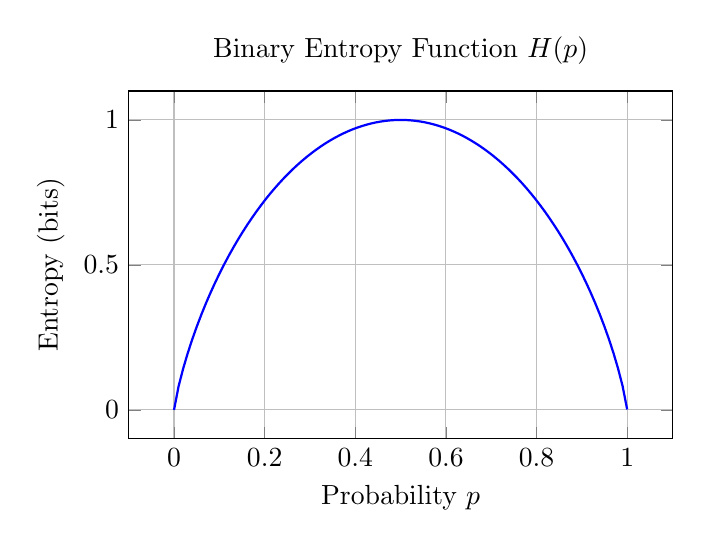
\begin{tikzpicture}
\begin{axis}[
    title={Binary Entropy Function $H(p)$},
    xlabel={Probability $p$},
    ylabel={Entropy (bits)},
    grid=major,
    width=0.7\textwidth,
    height=6cm
]
\addplot[blue, thick, domain=0:1, samples=100] {-x*log2(x) - (1-x)*log2(1-x)};
\end{axis}
\end{tikzpicture}
\end{center}

\subsection{Rate-Distortion Theory}
Rate-distortion theory deals with lossy compression. it defines the minimum rate $R(D)$ required to represent a source with a maximum allowable distortion $D$. This is the theoretical foundation for image (JPEG) and video (MPEG) compression.
